\documentclass[tikz,border=8pt]{standalone}
\usepackage{amsmath,amssymb}
\usetikzlibrary{arrows.meta,automata,positioning,quotes}
\begin{document}
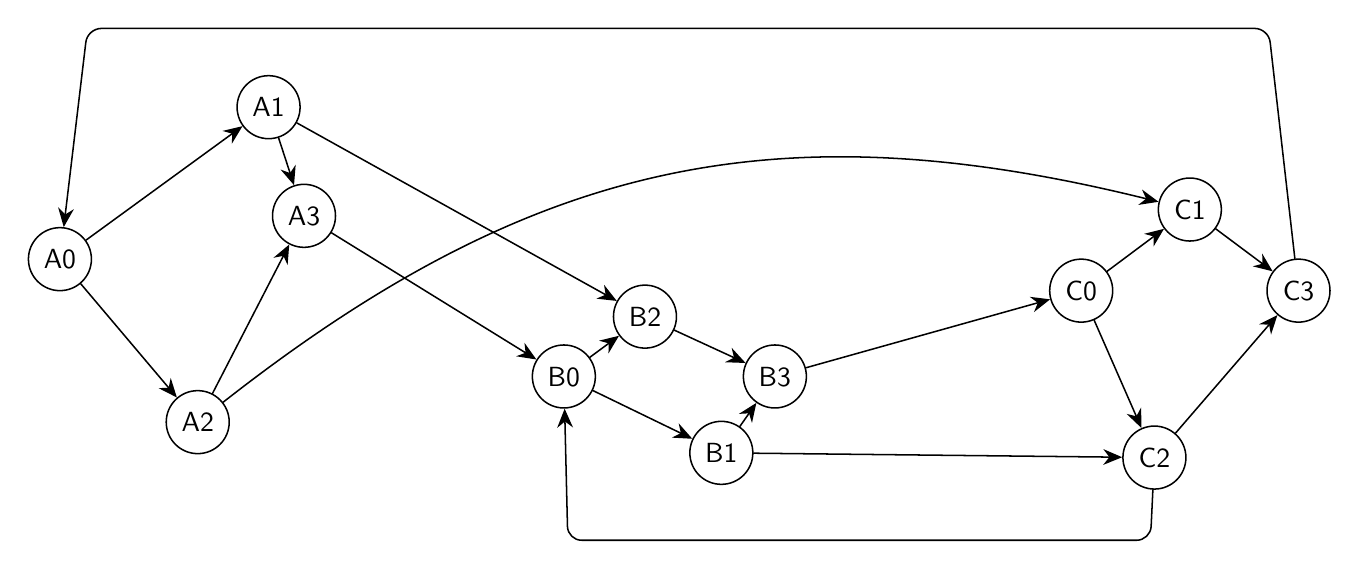
\begin{tikzpicture}[x=1cm,y=1cm]
\tikzset{
  graphnode/.style={circle,draw=black,line width=0.55pt,minimum size=8mm,inner sep=1pt,font=\sffamily},
  graphedge/.style={draw=black,line width=0.55pt,line cap=round,line join=round},
  directed/.style={graphedge,-{Stealth[length=2.4mm,width=2.0mm]}},
  undirected/.style={graphedge}
}
\node[graphnode] (n_A0) at (-8.20,0.72) {A0};
\node[graphnode] (n_A1) at (-5.55,2.65) {A1};
\node[graphnode] (n_A2) at (-6.45,-1.35) {A2};
\node[graphnode] (n_A3) at (-5.10,1.27) {A3};
\node[graphnode] (n_B0) at (-1.80,-0.77) {B0};
\node[graphnode] (n_B1) at (0.20,-1.74) {B1};
\node[graphnode] (n_B2) at (-0.77,-0.01) {B2};
\node[graphnode] (n_B3) at (0.88,-0.77) {B3};
\node[graphnode] (n_C0) at (4.77,0.32) {C0};
\node[graphnode] (n_C1) at (6.15,1.35) {C1};
\node[graphnode] (n_C2) at (5.70,-1.80) {C2};
\node[graphnode] (n_C3) at (7.53,0.32) {C3};
\draw[directed] (n_A0) -- (n_A1);
\draw[directed] (n_A0) -- (n_A2);
\draw[directed] (n_A1) -- (n_A3);
\draw[directed] (n_A2) -- (n_A3);
\draw[directed] (n_B0) -- (n_B1);
\draw[directed] (n_B0) -- (n_B2);
\draw[directed] (n_B1) -- (n_B3);
\draw[directed] (n_B2) -- (n_B3);
\draw[directed] (n_C0) -- (n_C1);
\draw[directed] (n_C0) -- (n_C2);
\draw[directed] (n_C1) -- (n_C3);
\draw[directed] (n_C2) -- (n_C3);
\draw[directed] (n_A3) -- (n_B0);
\draw[directed] (n_B3) -- (n_C0);
\draw[directed] (n_A1) -- (n_B2);
\draw[directed] (n_A2) to[bend left=26, looseness=1.05] (n_C1);
\draw[directed] (n_B1) -- (n_C2);
\draw[directed,rounded corners=5pt] (n_C3) -- (7.15,3.65) -- (-7.85,3.65) -- (n_A0);
\draw[directed,rounded corners=5pt] (n_C2) -- (5.65,-2.85) -- (-1.75,-2.85) -- (n_B0);
\end{tikzpicture}
\end{document}
